\section{Wednesday, November 6, 2019}
\subsection{Binary Heaps}
A \vocab{heap} is a data structure represented by an underlying array $A$ that can be interpreted as an ``almost complete" binary tree. Each node in the tree corresponds to a single element in the array. The tree is ``almost complete" in the sense that the tree is completely filled on all levels except possibly the lowest, which is filled from the left to right up to a point. 

How do we represent our almost complete binary tree with an array? We can start our array at index $1$ (using a sentinel at index $0$), and we can store the root of the node in \verb!A[1]!. Furthermore, given the index $i$ of a node, we can place the indices of its parent, left child, and right child in the indices $\floor{i/2}$, $2i$, and $2i + 1$, respectively. As an example, consider the following array:

\[\fbox{32} \sep \fbox{24} \sep \fbox{22} \sep \fbox{23} \sep \fbox{7} \sep \fbox{2} \]

\noindent The corresponding binary heap is presented below:

\begin{figure}[h]
\centering
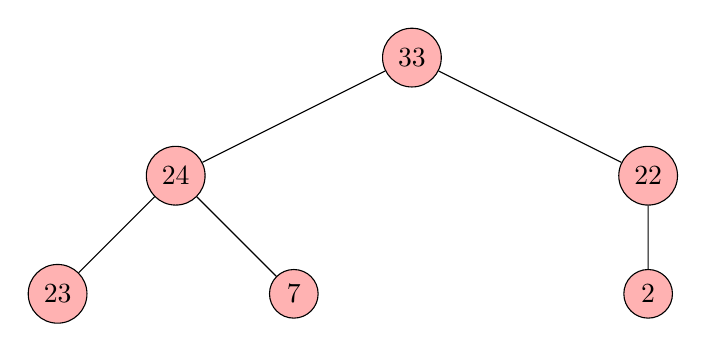
\begin{tikzpicture}[level/.style={sibling distance=60mm/#1}]
\node [circle,draw,fill=red!30] (z){$33$}
  child {node [circle,draw,fill=red!30] (a) {$24$}
    % child {node [circle,draw,fill=red!30} (b) {$23$}
    child {node [circle,draw,fill=red!30] (b) {$23$}
        }
        child {node [circle,draw,fill=red!30] (c) {$7$}
    }
    % child {node [circle,draw,fill=red!30] (g) {$4$}}
  }
    child {node [circle,draw,fill=red!30] (j) {$22$}
        child {node [circle,draw,fill=red!30] (k) {$2$}
        }
    % child {node [circle,draw,fill=red!30] (k) {$2$}
};
\end{tikzpicture}
\caption{A Binary Heap}
\end{figure}


For instance, observe that the parent of the nodes storing $24$ and $22$ is the node storing $33$. Furthermore, note that the the elements $24$ and $22$ are in the second and third indices of the array. By noting that $\floor{2/2} = \floor{3/2} = 1$, we see that the parent of these two nodes should be at index $1$, which agrees with our array representation above.

There are two types of binary heaps: \vocab{max-heaps} and \vocab{min-heaps}. In both cases, the nodes satisfy a \vocab{heap property}, which differs depending on the type of heap. In a max heap, the \vocab{max-heap property} asserts that for every node $v$ in the tree, we require \verb!A[PARENT(i)] >= A[i]!. On the other hand, in a min-heap property, we require \verb!A[PARENT(i)] <= A[i]!. In other words, the parent of a node in a max heap is always greater than or equal to the node itself, and the parent of a node in a min heap is always less than or equal to the node itself. Thus, we can conclude that the figure above is a max heap. 

Note that the max heap depicted above does not have its entire last level full. This is okay --- as we mentioned previously, the tree must be completely filled on all levels except possibly the lowest, which should be filled from the left to the right up to a point. \\

\newpage

\noindent Here is an example of a tree that is \textbf{not} a heap:


\begin{figure}[h]
\centering
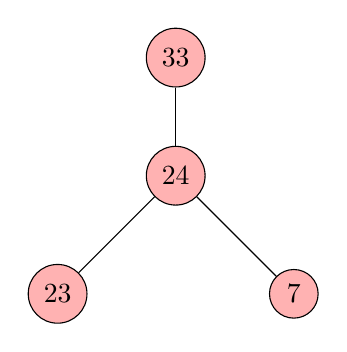
\begin{tikzpicture}[level/.style={sibling distance=60mm/#1}]
\node [circle,draw,fill=red!30] (z){$33$}
  child {node [circle,draw,fill=red!30] (a) {$24$}
    % child {node [circle,draw,fill=red!30} (b) {$23$}
    child {node [circle,draw,fill=red!30] (b) {$23$}
        }
        child {node [circle,draw,fill=red!30] (c) {$7$}
    }
    % child {node [circle,draw,fill=red!30] (g) {$4$}}
    % child {node [circle,draw,fill=red!30] (k) {$2$}
};
\end{tikzpicture}
\caption{Not a Binary Heap}
\end{figure}

Although the tree depicted above satisfies the max heap property (each parent is greater than its children), the level directly after the root node (with value $33$) is not completely filled, so it is invalid to begin the level after that. Thus, this is not a binary heap.

Due to the ``almost completeness" of binary heaps, we are ensured that the binary tree represented by the heap is balanced. In other words, the height of the binary tree grows logarithmically in the number of nodes (it's impossible for heaps to exhibit degeneracy).

We will now discuss how to insert and extract elements from min heaps. Although our descriptions will specify how to insert and extract elements from a min heap, they can easily be modified to insert and extract elements from a max heap. 

\subsubsection{Insertion}

When inserting an element into a min heap, we need to be careful not to mess up the min heap property. This can be done with the following insertion procedure:
\begin{enumerate}
    \item Insert the new element to the end of the array (so it will be the bottom right-most element in the tree).
    \item While the parent's key is larger than the inserted element's key, swap the parent node with the inserted element's node.
    \item Insertion is complete.
\end{enumerate}

For example, suppose we have the following min heap:

\begin{figure}[h]
\centering
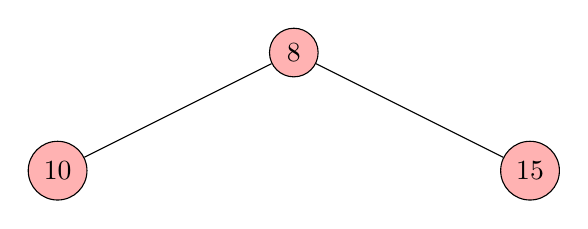
\begin{tikzpicture}[level/.style={sibling distance=60mm/#1}]
\node [circle,draw,fill=red!30] (z){$8$}
  child {node [circle,draw,fill=red!30] (a) {$10$}
    }
    child {node [circle,draw,fill=red!30] (b) {$15$}
    % child {node [circle,draw,fill=red!30] (g) {$4$}}
    % child {node [circle,draw,fill=red!30] (k) {$2$}
};
\end{tikzpicture}
\caption{Min Heap}
\end{figure}
If we wanted to add the node with key $5$ into the heap, we would first append the value to the last slot in the array (so $5$ would be a child of the node $10$). Subsequently, we would compare $5$ with $10$. Since $5 < 10$, we would swap the node $5$ with its parent node, and we would repeat the procedure so that $5$ is the root node, its immediate left child is $8$, whose immediate right child would be $10$. 

\begin{figure}[h]
\centering
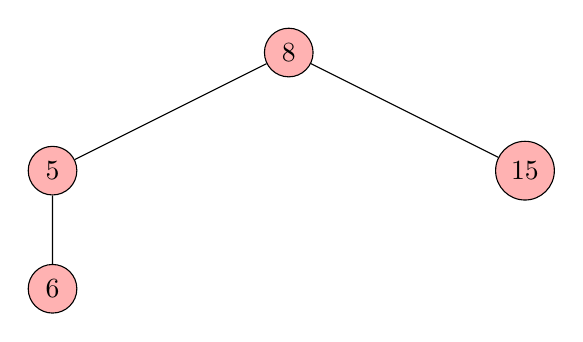
\begin{tikzpicture}[level/.style={sibling distance=60mm/#1}]
\node [circle,draw,fill=red!30] (z){$8$}
  child {node [circle,draw,fill=red!30] (a) {$5$}
      child {node [circle,draw,fill=red!30] (c) {$6$}
      }
    }
    child {node [circle,draw,fill=red!30] (b) {$15$}
    % child {node [circle,draw,fill=red!30] (g) {$4$}}
    % child {node [circle,draw,fill=red!30] (k) {$2$}
};
\end{tikzpicture}
\caption{Min Heap}
\end{figure}

\newpage

\subsubsection{Extraction}

What about deletion? When working with heaps, we do not extract any node other than the root. This allows us to get the smallest element (in a min heap) very quickly. But, how do we maintain the min heap property? This can be done with the following \verb!extractSmallest()! procedure:


\begin{enumerate}
    \item Replace the root with the smallest node in the tree (but store the value of the old root --- this is the value that we are extracting). We will henceforth refer to this new root as node $v$.
    \item Compare $v$ to both children. If $v$ is larger than either child (i.e. the min heap property is violated), then swap the root with the smallest child. Repeat the swapping procedure on the subtree rooted at $v$ until $v$ is smaller than both of its children. At this point, the min heap property will be satisfied.
\end{enumerate}


